\section{Background \label{sec:Background}}

 \subsection{IEEE~802.11 ah networks and \gls{raw} \label{subsec:80211ah_raw}}

% \begin{figure}[t]
%   \centering
%   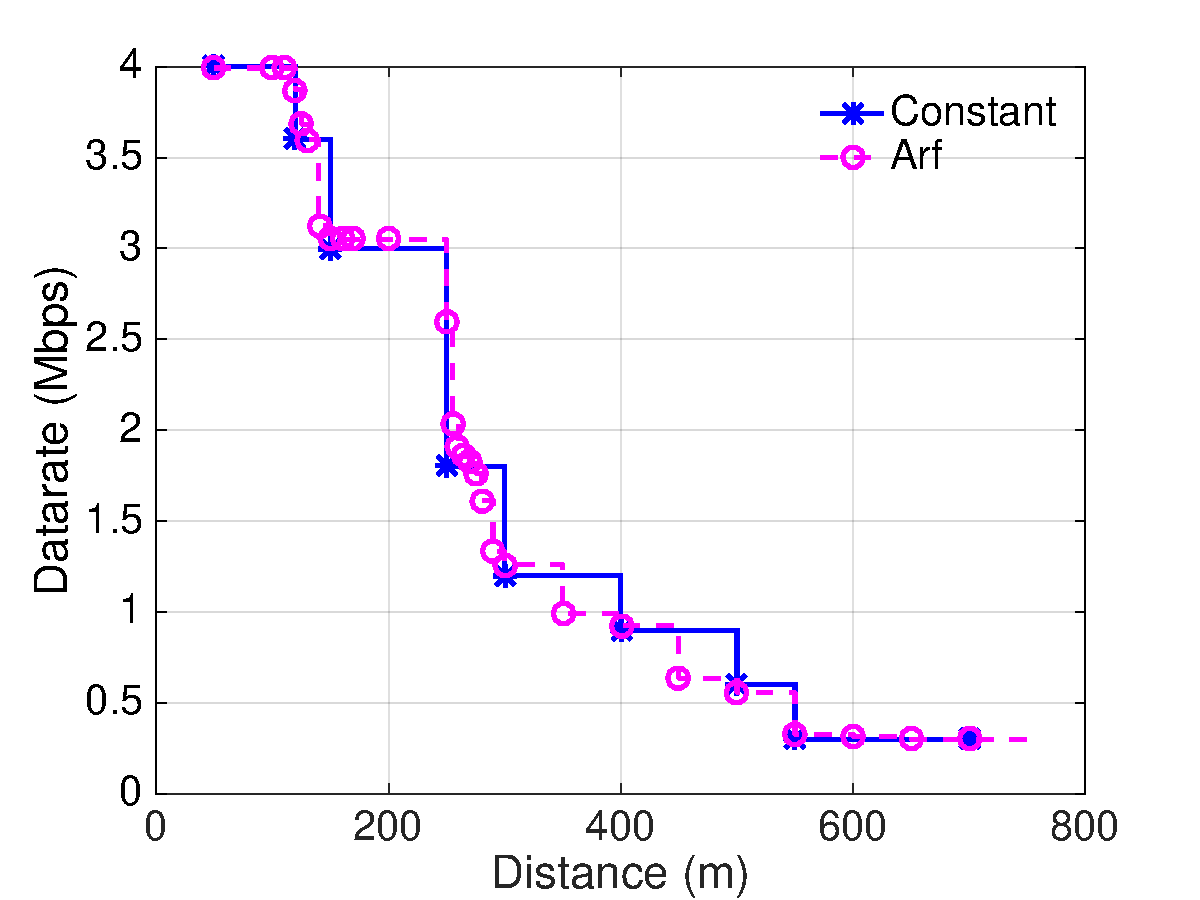
\includegraphics[width=0.45\textwidth]{figures/distance-datarate-512bytes}  \caption{The used transmission data rate for different distance. \label{fig:dist-datarate}}
% \end{figure}


\begin{table}[t]
\centering
\caption{802.11ah MCSs for 1, 2~MHz, NSS=1, GI=$8~\mu{}s$}
\label{tab:wifi-modes}
\begin{tabular}{ccccc}
\hline
\multirow{2}{*}{\begin{tabular}[c]{@{}c@{}}MCS\\ Index\end{tabular}} & \multirow{2}{*}{Modulation} & \multirow{2}{*}{\begin{tabular}[c]{@{}c@{}}Coding \\ rate\end{tabular}} & \multicolumn{2}{l}{Data rate (Kbps)} \\ \cline{4-5} 
 &  &  & 1 Mhz & 2 Mhz \\ \hline
0 & BPSK & 1/2 & 300 & 650 \\ 
1 & QPSK & 1/2 & 600 & 1300 \\ 
2 & QPSK & 3/4 & 900 & 1950 \\ 
3 & 16-QAM & 1/2 & 1200 & 2600 \\ 
4 & 16-QAM & 3/4 & 1800 & 3900 \\ 
5 & 64-QAM & 2/3 & 2400 & 5200 \\ 
6 & 64-QAM & 3/4 & 2700 & 5850 \\ 
7 & 64-QAM & 5/6 & 3000 & 6500 \\ 
8 & 256-QAM & 3/4 & 3600 & 7800 \\ 
9 & 256-QAM & 5/6 & 4000 & Not valid \\ 
\multirow{2}{*}{10} & \multirow{2}{*}{BPSK} & 1/2 with 2x & \multirow{2}{*}{150} & \multirow{2}{*}{Not valid} \\
 & & repetition & & \\ \hline
\end{tabular}
\end{table}

In this section, we provide an overview of the \gls{raw}, the IEEE~802.11ah network and its typical settings on the physical and MAC layers. 
%A surrogate \gls{raw} model for such network scenarios is subsequently built to accurately predict the performance.


%simulation environment parameters used during training. 
%Since \gls{raw} is scalable under uplink traffic, 

IEEE~802.11ah mainly targets \gls{iot} network scenarios, where sensors (stations) are randomly placed around the AP within a maximum radius, periodically monitor the environment and send the resulting data to a server (via the \gls{ap}). Like the legacy IEEE~802.11 technologies, at the physical layer, IEEE~802.11ah supports multiple transmission data rates represented by the MCSs. The stations are allowed to dynamically choose the MCS for packet transmission to adapt to the conditions of the wireless channel. As listed in Table \ref{tab:wifi-modes}, the number of supported MCSs depends on the channel width. For channel bandwidth 1 MHz,  MCS 0$-$10 are supported with transmission data rates ranging from 150 Kbps to 4 Mbps, and for 2 Mhz, MCS 0$-$9 are supported with transmission data rates ranging from 650 Kbps to 7.8 Mbps, more details can be found in \cite{80211ahStd}. At every beacon interval, the \gls{ap} broadcasts beacon frame carrying a \gls{rps} information element that specifies the \gls{raw} parameter configurations. Stations retrieve such \gls{raw} information from the beacon frame and access the channel only during their assigned \gls{raw} slot. 
%In order to obtain high performance, there is a need to build a \gls{raw} model that can accurately predict the performance under a variety \gls{raw} parameter values and network conditions.


The \gls{raw} information is carried in the \gls{rps} element, it specifies the stations belonging to the group, the number of slots, slot format and slot duration count sub-fields, which jointly determine the \gls{raw} slot duration as follows \cite{80211ahStd}: 
%\textcolor{red}{\cite{80211ahStd}}: 
\begin{equation} \label{eq:Duration}
D = 500~\mu{}s + C \times 120~\mu{}s  
\end{equation}
where $C$ represents \textit{slot duration count} sub-field, which is either $y = 11$ or $y = 8$ bits long if the slot format sub-field is set to respectively $1$ or $0$. The \textit{number of slots} field is $14-y$ bits long. When $y = 11$, each RAW consists of at most 8 slots and the maximum value of $C$ is $2^{11}-1=2047$, in this case the slot duration is up to $246.14$~ms. Otherwise, each RAW consists of at most 64 slots and the maximum value of $C$ is $2^{8}-1=255$, the slot duration is thus limited to $31.1$~ms. The \gls{raw} group duration is the sum of its slot durations.



% Besides \gls{raw}, there are numerous parameters involved in the physical and MAC layer of IEEE~802.11ah networks.
% %while we mainly focus on the most commonly used scenarios where
% In our experiments, we use the typical parameter settings, 
% as shown in Table~\ref{tab:ns3 parameters}. Given the low-power nature of battery powered sensors, the physical layer parameters are configured based on the low-power 802.11ah radio hardware prototype developed by Ba et al.~\cite{Ba2016}, with a transmission power of 0~dBm, a gain of 0~dBi (for both sensor and \gls{ap}), and noise figure of 6.8~dB. With such physical layer setting, the coverage of the networks is up to 500 meters based on the physical layer performance evaluation in \cite{bellekens2017outdoor}. As the \gls{iot} applications have relatively small payload size, packet size is assumed to be between  32 and 512 bytes.


% For each experimented scenario, we assume a coverage range to be $[d^-, d^+]  \subseteq [0, 500] $  meters and a packet size range to be $[ps^-, ps^+] \subseteq [32, 512] $ bytes. Each station $s$ randomly and uniformly chooses a value $d_s \in [d^-, d^+]$ as its distance to the \gls{ap}, and an integer value $ps_s \in [ps^-, ps^+]$ as its packet size. Based on its distance to the \gls{ap} $d_s$, the station $s$ uses the corresponding MCS for packet transmission according to the rate control method. Several rate control methods have been proposed and used on the real devices for legacy IEEE~802.11 to select the appropriate MCS for packet transmission, for example, Arf \cite{arf1997},  Aarf \cite{aarf2004}, Onoe \cite{Onoe} and Minstrel \cite{minstrel}. For the IEEE~802.11ah network, we use a simpler rate control method, allowing the stations to select the MCS solely based on its distance to the \gls{ap}, i.e., choosing the MCS which can stably achieve the maximal throughput at a certain distance, as shown in Figure \ref{fig:dist-datarate}. The size of the stations' transmit queues is configured to be 10 packets. 
% %For training simplicity, we assume each station sends one packet per second, the built model can be further used by the \gls{raw} optimization algorithms, such as \gls{taora} \cite{Sensor2017,Sensys2017},  to calculate \gls{raw} performance under arbitrary data transmission intervals.



% % As the \gls{iot} applications have relatively small payload size, we limit the packet size range $[\underline{ps}, \bar{ps}] $ to $[32, 512]$,  choose 500 meters as the maximum distance between stations and the \gls{ap} based on the physical layer performance evaluation in \cite{bellekens2017outdoor}.

% %Each experiment runs for 60 seconds of simulated time. As \gls{raw} is configured in each beacon interval of 204.8~ms, the results of every simulated configuration are averaged over 290 beacon intervals, ensuring the generality of the trained model.



% %As the RAW optimization algorithm proposed in Section~\ref{sec:algorithm} groups together stations that use the same \gls{mcs}, the model assumes a fixed \gls{mcs}. However, as \gls{raw} performance depends on the \gls{mcs} used, a different model is to be trained for each \gls{mcs} that stations are expected to use. We illustrate this by developing a separate a high-throughput (HT) and low-throughput (LT) model for two different \gls{mcs} parameter sets. This can be trivially extended to other \gls{mcs} values. 


% \begin{table}[t]
% \centering
% \renewcommand{\arraystretch}{1.2}
% %\tiny
% \caption{\textsc{Simulation parameters used during training}\label{tab:ns3 parameters}}
% \begin{tabular}{ll}
% \hline
% \textbf{PHY parameters}             & \textbf{Value}  \\
% \hline
% %Frequency (Mhz)                      & 868 \\
% TX power (dBm)             & 0    \\
% TX/RX gain (dB)                        & 0     \\
% Noise Figure (dB)               & 6.8      \\  
% %Coding method                  & BCC \\
% Propagation model         & Outdoor \\ %, macro~\cite{Hazmi2012} \\
% Error rate model               & YansErrorRate \\
% \hline
% \textbf{MAC parameters}               & \textbf{Value}  \\
% \hline
% % CWmin                          & 15 \\
% % CWmax                          & 1023      \\
% %Duration of AIFS (us)\textcolor{red}{change to DIFS}            & 316      \\
% Traffic access categories             & \textcolor{black}{ AC\_{BE} } \\
% Duration of AIFS ($\mu$s)             & 264      \\
% Duration of SIFS ($\mu$s)            & 160      \\
% %RTS/CTS                        & not enabled  \\
% Beacon interval (ms)           & 204.8 \\
% %Cross slot boundary            & Enabled \\
% %Rate control algorithm         & constant  \\
% Size of transmission queue (packets)  & 10  \\
% Packet transmission interval (s)        & 1  \\
% Station distribution           & random  \\
% Rate control algorithm                     & XXX \\
% %Average payload size (bytes)           & 64   \\
% %Topology radius (m)     & 200  \\
% \hline
% \end{tabular}
% \end{table}
 
 
\subsection{Related Work \label{subsec:related_work}}


As the IEEE~802.11ah standard does not specify how to configure the actual \gls{raw} grouping parameters, several studies have been conducted on \gls{raw} performance evaluation, modeling and optimization. Raeesi et al. evaluated  \gls{raw} performance using the network simulator OMNeT++, the results demonstrate that the RAW feature provides
substantial performance (i.e., throughput, energy consumption and latency) improvements, in particular in scenarios where there is a relatively high number of collisions and heavily loaded network \cite{Raeesi2014a}. Using an IEEE~802.11ah implementation in ns-3
\cite{WNS32016}, we further evaluated the optimal \gls{raw}  configuration under a variety of network conditions, such as traffic load, number of stations, and traffic distribution among stations~\cite{WoWMoM2016}. These works highlight the impact of network conditions on the optimal \gls{raw} configurations, demonstrate there is a need for a \gls{RAW} performance model, which can predict performance for the given RAW parameter values (e.g., number of groups and slots, group duration, station assignment) and given the current network conditions (e.g., network topology, traffic load, station number). In addition, the \gls{raw} model should be enable to be applicable in real time for \gls{raw} optimization under dynamic network conditions.


%\subsection{\gls{raw} performance models}

%In order to allow the AP to choose the optimal RAW configuration in real-time, a RAW performance model is needed. Given the current network conditions (e.g., network topology, traffic) and a set of RAW parameter values (e.g., number of groups and slots, group duration, station assignment) the model should estimate performance (e.g., in terms of throughput). 

Several mathematical \gls{raw} models have been proposed to calculate  performance under specific network and traffic conditions. These models make use of different techniques, such as probability theory~\cite{Wang2015}, Markov chains~\cite{Raeesi2014a, Khorov2015b,Zheng2014, Evgeny2018, Khorov2015b, Park2014b}, and maximum likelihood estimation~\cite{Park2014b}. Some models  assume stations have infinite packets to send (i.e., saturated model)  \cite{Raeesi2014a, Zheng2014, Park2014b, Evgeny2018}. The works of \cite{Raeesi2014a, Zheng2014, Park2014b} are based on the Bianchi model \cite{bianchi2000performance}, which is a classical mathematical model of the \gls{dcf} for the legacy IEEE~802.11 networks. It utilizes the Markov Chain theory, assumes the network is always in the steady state and saturated mode. Raeesi \textit{et al.}  update the Bianchi model to calculate the probability of collisions inside a \gls{raw} slot without taking into account the finite length of the RAW slot \cite{Raeesi2014a}. Zheng \textit{et al.} extended the Bianchi model to support \gls{raw} considering both cross and non-cross slot boundary traffic, the extended model is able to calculate the throughput with any given number of stations and \gls{raw} duration~\cite{Zheng2014}. Park \textit{et al.} adopt the Bianchi model for the  joint usage of the PS-Poll and RAW mechanisms, and determine the duration of \gls{raw} groups in order to achieve the maximal successful transmission probability for a given number of stations~\cite{Park2014b}. A more accurate mathematical model is recently developed by Lyakhov \textit{et al.} \cite{Evgeny2018}, by taking into account the non-steady state of the backoff function at the beginning of the RAW. Wang \textit{et al.} \cite{Wang2015} , as well as Khorov \cite{Khorov2015b}, proposed none saturated model for low power \gls{iot}, assuming each station sends one packet per \gls{raw} slot interval. By taking into account the reset of the backoff function state at the beginning of the RAW slot, Khorov \textit{et al.} presented a model to calculate the successful packet transmission probability for a certain \gls{raw} group duration~\cite{Khorov2015b}, while Wang's model mainly focus on energy consumption~\cite{Wang2015}. 

The above mathematical models have two main disadvantages. \todo {First of all, these models are computationally hard}. This makes it infeasible to execute them in real-time on actual \gls{ap} hardware, where at most a few milliseconds are available at the start of the beacon interval to calculate a new \gls{raw} configuration. More importantly, they assume certain types of traffic and ideal channel conditions, without communication errors, delays or capture effects. The combination of these factors make such models useful only from a theoretical point of view, to analyze the effectiveness of \gls{raw} under a variety of conditions. However, they cannot be used for real-time station grouping under dynamic and realistic traffic conditions. 
Chang \textitet{et al.} made a step further, to support more diverse traffic demands \cite{Chang2018}. They use the results of two extreme cases (i.e., with infinite traffic and with only a single packet) to extrapolate a regression-based analytical model that can accurately fits the contention success probability of any traffic patterns. However, the regression model does not take the finite length of the RAW slot into account.
 Recently, we proposed a new RAW performance model based on supervised surrogate modeling \cite{wowmom2018}. The model is trained on a limited set of labeled data samples from ns-3 simulation results, support realistic channel conditions, including communication errors, propagation delays and capture effects. However, both of the model of Change \cite{Chang2018} and our previous work \cite{wowmom2018}, only support homogeneous networks (i.e., all stations use the same MCS and average packet size). 
 
 
 
 In this paper, we present a novel training methodology for surrogate modeling of IEEE~802.11ah heterogeneous network. It uses average transmission time, i.e., the total packet transmission time of a heterogeneous network averaged over all the sent packets, as an input parameter of the surrogate model, and packet receiving rate as the output parameter of the surrogate model. This results in highly reduced design space, allowing the model to be accurately trained with only a few labelled sample data points. 



% Based on the proposed \gls{raw} models, \cite{Chang2018} and \cite{wowmom2018} also developed the \gls{raw} optimization algorithms.  \cite{Chang2018} presents a traffic-aware station grouping algorithm to maximize the \gls{raw} performance. However, due to the drawbacks of the model, the algorithm assumes the number of \gls{raw} groups and \gls{raw} duration are predetermined, which is actually part of the \gls{raw} optimization problem and need to be solved.
% In \cite{wowmom2018}, we present a real-time \gls{raw} optimization algorithm, called \gls{moroa}, supporting a wide range of traffic conditions and heterogeneous stations. However, since the model itself only support stations with same MCS and  packet sizes, the \gls{moroa} only allows same type of stations within a single \gls{raw} group. This limited the flexibility of the algorithm in finding an optimal RAW configuration.




%Moreover, it is very fast to evaluate once trained, allowing it to be used for real-time RAW parameter optimization.




% In addition, a traffic-aware station grouping algorithm was proposed based on the model. However, it assumes the number of \gls{raw} groups and \gls{raw} duration are predetermined, which is actually part of the \gls{raw} optimization problem and need to be solved. The \gls{taroa} algorithm ~\cite{Sensor2017,Sensys2017} can adapt the optimal \gls{raw} parameters in real-time by estimating the current traffic conditions, based solely on information available at the \gls{ap}. However, it derives the optimal number of stations to assign to a group based on saturated state simulation results. Both \cite{Chang2018} and ~\cite{Sensor2017,Sensys2017} only support homogeneous stations (i.e., all stations use the same MCS and average packet size). 

% Recently, we proposed a surrogate model of \gls{raw} which are trained using realistic simulation results, and a real-time \gls{raw} optimization algorithm based on the model, called \gls{moroa}, was proposed supporting a wide range of traffic conditions and heterogeneous stations \cite{wowmom2018}. 
% However, the model itself only support stations with same MCS and  packet sizes, which only allows same type of stations within a single \gls{raw} group, and limited the flexibility of the algorithm in finding an optimal RAW configuration.



%  However, the existing analytical models are computationally expensive and unrealistic due to their assumptions.
 
%  Although a surrogate \gls{raw} model is constructed in \cite{wowmom2018}, it only supports stations with the same \gls{mcs} and packet size, the lack of support on adaptive rate control and diverse packet size make it inapplicable to the realistic scenarios.



%Instead of using Binary Exponential Backoff (BEB) scheme inside of \gls{raw} group, Gopinath \textitet{et al.} proposed a new backoff scheme using an appropriate integer sequences for calculating new Contention Window, and  developed an analytical model  for computing saturated throughput \cite{gopinath2018mathematical}.




% This is not a very realistic assumption for \gls{iot} and \gls{mtc}~\cite{Khorov2015b}. Those models cannot be directly applied to an IoT network, in which each sensor generates traffic periodically. 













% models to estimate the contention success probabilities of the two extreme cases (i.e., with infinite traffic and with only a single packet), and then use the estimates of the two cases to 
















% \subsection{\gls{raw} optimization algorithms}

% In addition to modeling \gls{raw} performance, several algorithms have been proposed to optimize \gls{raw} performance. Some of them group stations based on very simple metrics  \cite{Chang2015, Qutab-Ud-Din2015, Ogawa2013}. Chang \textit{et al.} proposed a set partitioning algorithm that assumes the (static) traffic demand of each station is known by the \gls{ap} and load balances them across groups~\cite{Chang2015}. While stations are grouped based on fully random random AIFSN  ~\cite{Ogawa2013}, or back-off timer value~\cite{Qutab-Ud-Din2015} which is unknown to the \gls{ap} in reality. They all assume the number of \gls{raw} slots and groups is predetermined.






% allowing it to be used for real-time RAW
% parameter optimization.

% by using generic and flexible surrogate models, we present the \gls{moroa}  algorithm, which supports a wide range of traffic conditions and heterogeneous stations.





% This results in significant performance improvements, especially under non-saturated conditions, which are prevalent in \gls{iot} and \gls{mtc} scenarios. 




% However, it still has two shortcomings that can be addressed. First, it derives the optimal number of stations to assign to a group based on saturated state simulation results. Second, it only supports homogeneous stations (i.e., all stations use the same MCS and average packet size). 



% Their simplicity makes it computationally feasible to deploy them in real networks. 

% it is necessary to use this information in real-time, in order to optimize \gls{raw} parameters in an actual network.




% %Several algorithms utilize \gls{raw} to mitigate hidden node collisions by splitting mutually hidden nodes into orthogonal groups~\cite{Yoon2016,Damayanti2016}%{Yoon2016,Dong2016,Damayanti2016}. 





% \cite{Chang2018} 

% Such set partitioning algorithms have several shortcomings. 


% First, high channel contention exists in dense sensor network even without the presence of hidden nodes. Reducing hidden nodes can mitigate collisions to some extent, but is not sufficient. 

% Second, they expect all information, such as the exact traffic intensity of each station, to be readily available at the \gls{ap} side, which in reality is not the case. Third, they assume that the number of groups and slots as well as their duration are predefined, and only the partitioning of stations among them needs to be solved. The number of groups and their duration, however, significantly influence \gls{raw} optimality~\cite{WoWMoM2016}. Finally, none of the presented algorithms take into account traffic dynamics. In a real network, the upstream traffic intensity of stations may change over time for a variety of reasons, and the algorithm should therefore adapt to these changes.

% Recently, we proposed the \gls{taroa}~\cite{Sensor2017,Sensys2017}. It adapts the optimal \gls{raw} parameters in real-time by estimating the current traffic conditions, based solely on information available at the \gls{ap}. However, it still has two shortcomings that can be addressed. First, it derives the optimal number of stations to assign to a group based on saturated state simulation results. Second, it only supports homogeneous stations (i.e., all stations use the same MCS and average packet size). 

% In this paper we present an improved algorithm, called \gls{moroa}, which supports a wide range of traffic conditions and heterogeneous stations, by using generic and flexible surrogate models. This results in significant performance improvements, especially under non-saturated conditions, which are prevalent in \gls{iot} and \gls{mtc} scenarios. 

% %use the simulation results (since the analytic model \cite{Zheng2014} does not support capture effect) of saturated state to derive the optimal number of stations $\sigma^r_\textit{opt}$, while in most case network is not saturated. Second, it can only support homogeneous station, i.e., all station have the same MCS and packet size.


% % In contrast to other state-of-the-art algorithms it is capable of adjusting its \gls{raw} configuration in real-time, in face of station and traffic dynamics. Furthermore, by exploiting the “more data” header field \textcolor{white}{and cross slot boundary} feature, a more accurate traffic estimation technique for IEEE 802.11ah sensor stations was proposed, which is integrated into an enhanced version of the Traffic-Adaptive \gls{raw} Optimization Algorithm, referred to as E-TAROA \cite{Sensys2017}. With more accurate traffic estimation in very dense networks with thousands of sensor stations, E-TAROA results in a significantly more optimal \gls{raw} configuration. Specifically, E-TAROA converges significantly faster and achieves up to 23\% higher throughput and 77\% lower latency than the original TAROA algorithm under high traffic loads.



